\documentclass{standalone}

\usepackage{tikz}
\usetikzlibrary{hobby, decorations.markings, decorations.pathreplacing,shapes.misc,arrows.meta}

\begin{document}
\tikzset{% adapted from hobby_doc.tex
  show curve controls/.style={
    decoration={
      show path construction,
      curveto code={
        \draw [blue, -{Circle[black,open]}] (\tikzinputsegmentfirst) -- (\tikzinputsegmentsupporta) ;
        \draw [blue, {Circle[black,open]}-] (\tikzinputsegmentsupportb) -- (\tikzinputsegmentlast) ;
      }
    },decorate
  },
}
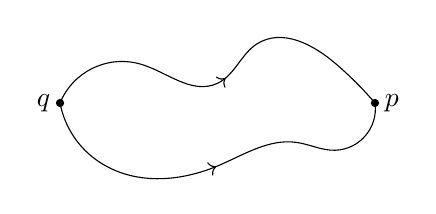
\begin{tikzpicture}[use Hobby shortcut, decoration={
	markings,
	mark=at position 0.5 with {\arrow{>}}}
]
	\coordinate[label=left:$q$] (q) at (0,0);
	\coordinate[label=right:$p$] (p) at (4,0);
	\draw[postaction={decorate}] (q) .. (1,0.5) .. (2,0.25) .. (2.5,0.75) .. (3.5, 0.5) .. (p);
	\draw[postaction={decorate}] (q) .. (0.5,-0.75) .. (2,-0.8) .. (3.0,-0.50) .. (3.5, -0.6) .. (p);
	\fill (q) circle (1.5pt);
	\fill (p) circle (1.5pt);
\end{tikzpicture}
\end{document}
